\chapter{Experiments}

In this chapter, we explain the setup of our experiments, describe how we measure the performance of different methods, and present the results.
All experiments were performed on a laptop with a 10-core, 16-thread Intel Core i7-12650H CPU and 32 GB of RAM. As for the software, Windows 11 24H2 was the operating system, MSVC 19.43 was the C++ compiler, and Python 3.12 was used.

\section{Datasets}

Here we briefly describe all datasets provided with the Google Hash Code Traffic signalling problem. This is important because the datasets have different sizes and structures.

\paragraph{A - An example: 4 parameters} Simple toy problem dataset used for debugging (See Figure~\ref{fig:hashcode_dataset_a}).

\paragraph{B - By the ocean: 5,974 parameters} Dataset based on a real city plan of Lisbon, Portugal (See Figure~\ref{fig:hashcode_dataset_b}).

\paragraph{C - Checkmate: 14,008 parameters} Dataset with a chessboard-like pattern and regular structure of intersections and streets (See Figure~\ref{fig:hashcode_dataset_c_e}).

% https://codeforces.com/blog/entry/88188#comment-765574
\paragraph{D - Daily commute: 167,748 parameters} By far the largest dataset with a challenging-to-navigate network from the \textit{Barabási-Albert} distribution.

\paragraph{E - Etoile: 1,386 parameters} Nicknamed \textit{Etoile}\footnote{\textit{Étoile} means star in French.}, this dataset is a one big star, meaning there is one very important intersection in the middle with hundrets of incoming streets (See Figure~\ref{fig:hashcode_dataset_c_e}).

\paragraph{F - Forever jammed: 10,002 parameters} Medium sized dataset but again with a complex network difficult to optimize.

\begin{figure}
    \centering
    % 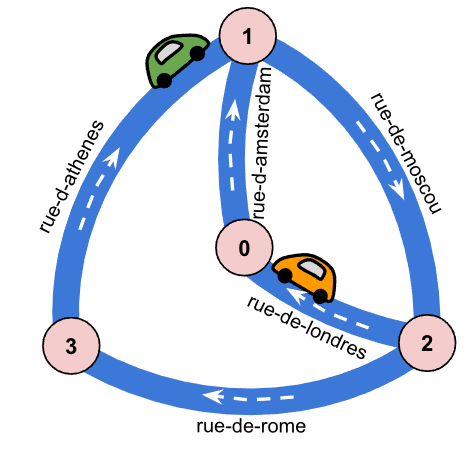
\includegraphics[width=\linewidth]{img/hashcode/figure5.png}
    % 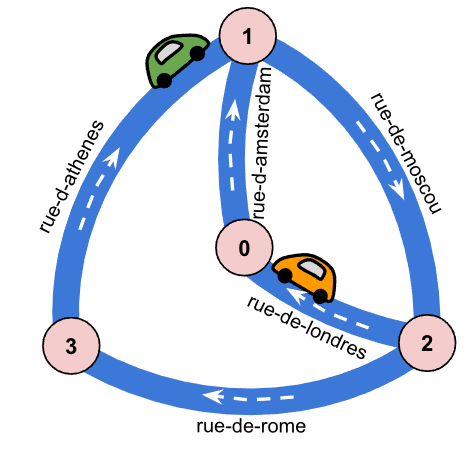
\includegraphics[width=.6\linewidth]{img/hashcode/figure5.png}
    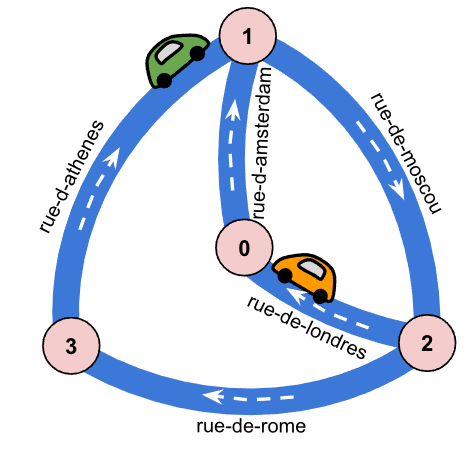
\includegraphics[width=.5\linewidth]{img/hashcode/figure5.png}
    \caption[Dataset A]{
        Dataset A \cite{google2023google}.
    }
    \label{fig:hashcode_dataset_a}
\end{figure}

\begin{figure}
    \centering
    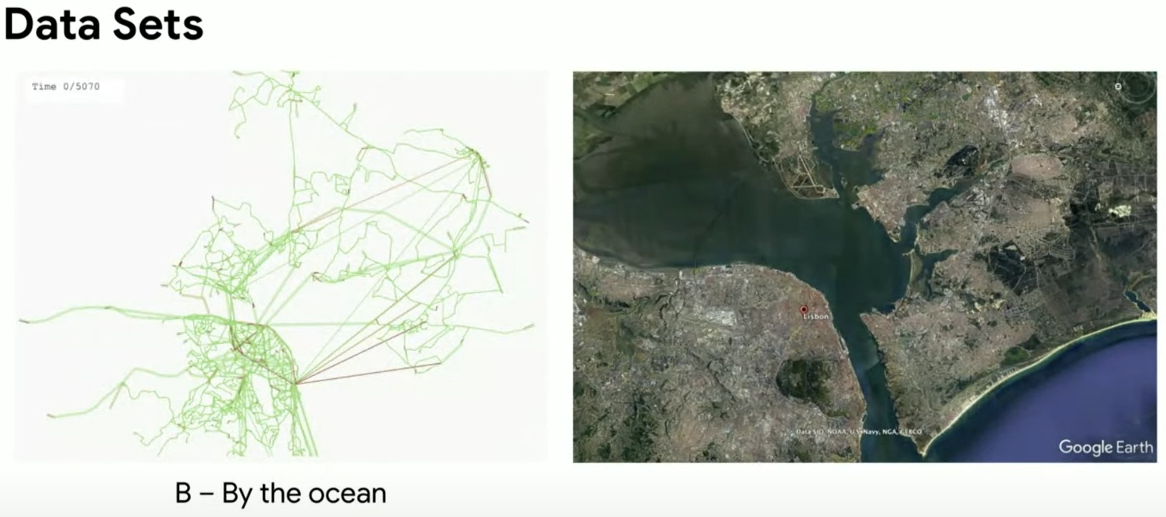
\includegraphics[width=\linewidth]{img/screenshots/hashcode_datasets_b.png}
    % 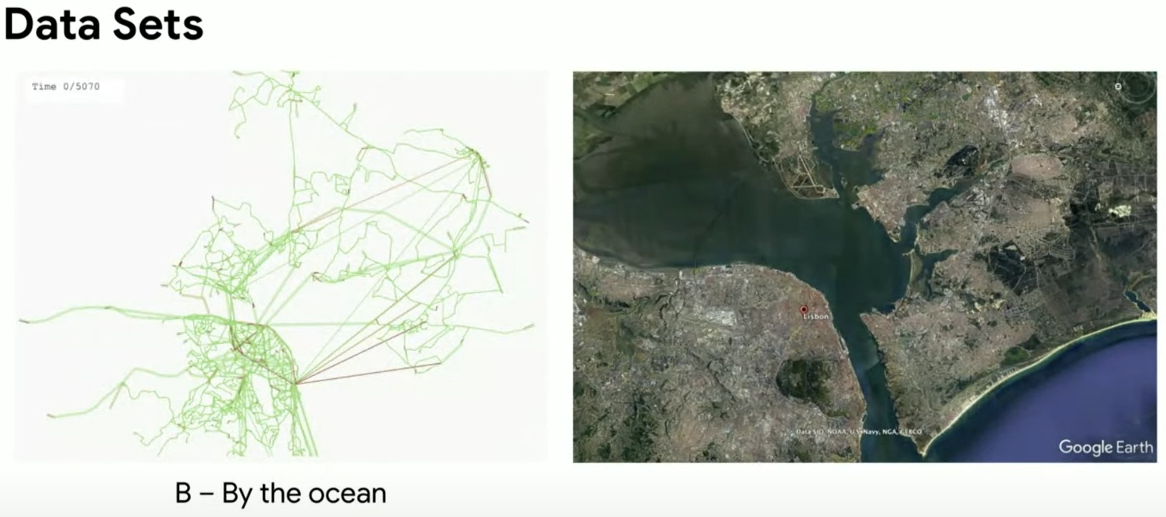
\includegraphics[width=.8\linewidth]{img/screenshots/hashcode_datasets_b.png}
    \caption[Dataset B]{
        Dataset B based on the real data of Lisbon on the right\footnotemark.
    }
    \label{fig:hashcode_dataset_b}
\end{figure}

\footnotetext{Screenshot from \href{https://www.youtube.com/watch?v=YPOVd-hQUjA}{Hash Code 2021: Online Qualification Round Livestream}.}

\begin{figure}
    \centering
    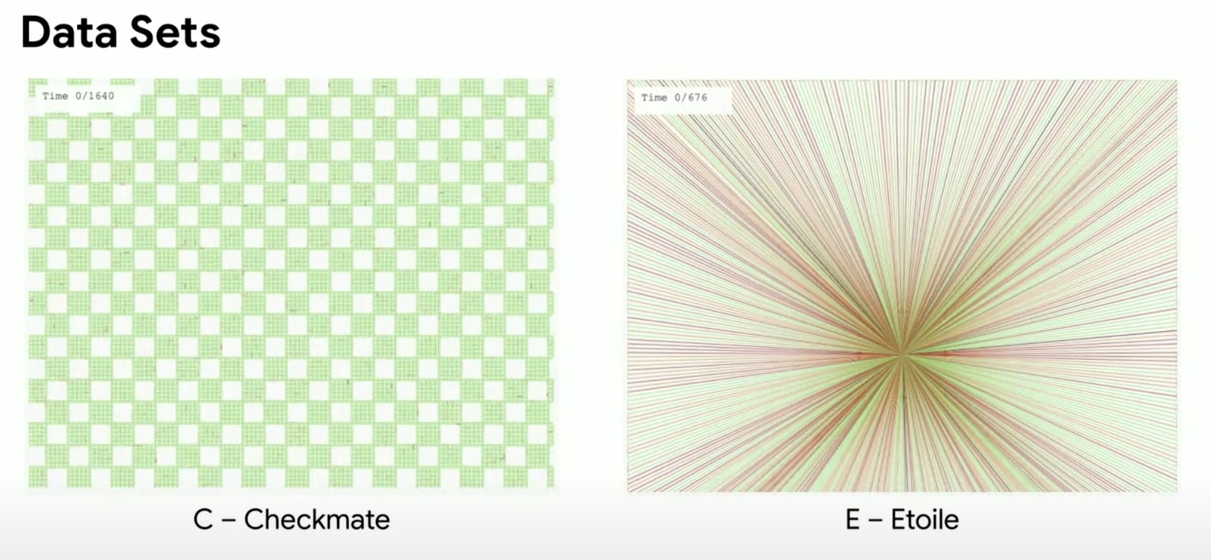
\includegraphics[width=\linewidth]{img/screenshots/hashcode_datasets_c_e.png}
    % 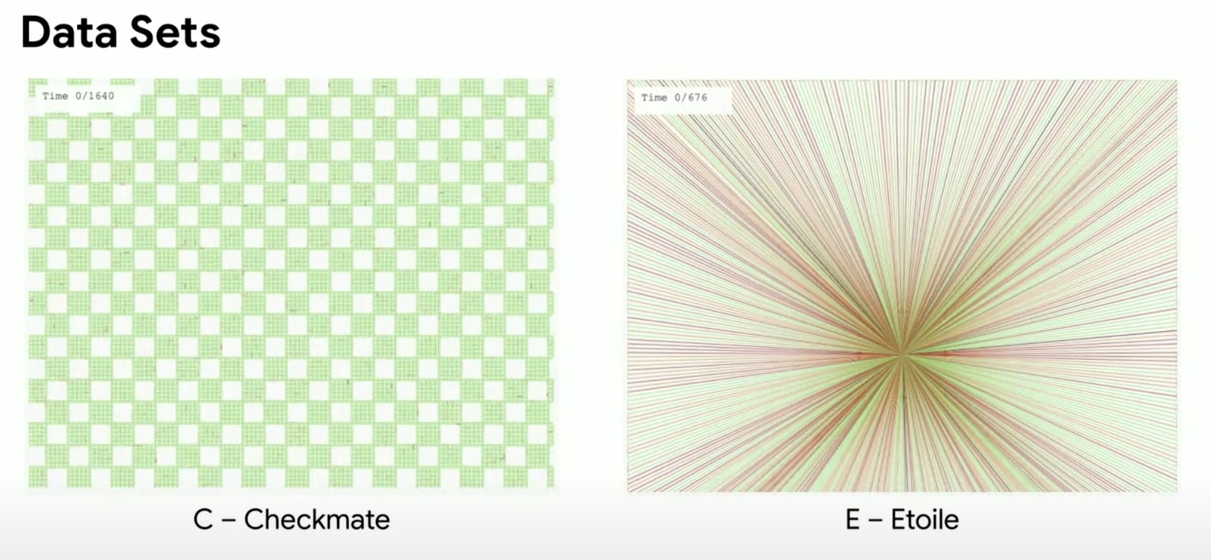
\includegraphics[width=.8\linewidth]{img/screenshots/hashcode_datasets_c_e.png}
    \caption[Datasets C and E]{
        Datasets C and E\footnotemark.
        }
        \label{fig:hashcode_dataset_c_e}
    \end{figure}
    
\footnotetext{See previous footnote.}

\bigskip

As previously stated, each dataset yields an absolute score in different range. To compare the performance across all datasets, we normalize the scores to a 0--1 range. 0 is a baseline solution with default order and default times and 1 is the maximum known score for the dataset. Note that the baseline is already a good solution and there may not be much room to improve further e.g., in dataset B.

\section{Experiment 1: Initialization}

In the first experiment, we compare the performance of different initialization methods across all datasets. The goal is to figure out how much we can improve the baseline solution and which initialization method to use for further optimization.

\subsection*{Methodology}

We compare three initialization methods: \textit{adaptive}---adaptive order and default times, \textit{random}---random order and default times, and \textit{scaled}---default order and scaled times. Since the random method is stochastic, it was run 100 times and averaged. The rest of the methods are deterministic and therefore run only once.

\subsection*{Results}

The results are shown in Figure~\ref{fig:init_experiment}. Overall, the adaptive method provides the biggest improvement over the baseline. It also yields a really high score for the largest dataset D. The only exception is the dataset F, where the otherwise mediocre scaled method performs really well. The random method generally performs the same as the baseline but it can still be a good initialization starting point if we care about variety and randomness in the solution. 

\begin{figure}
    \centering
    % 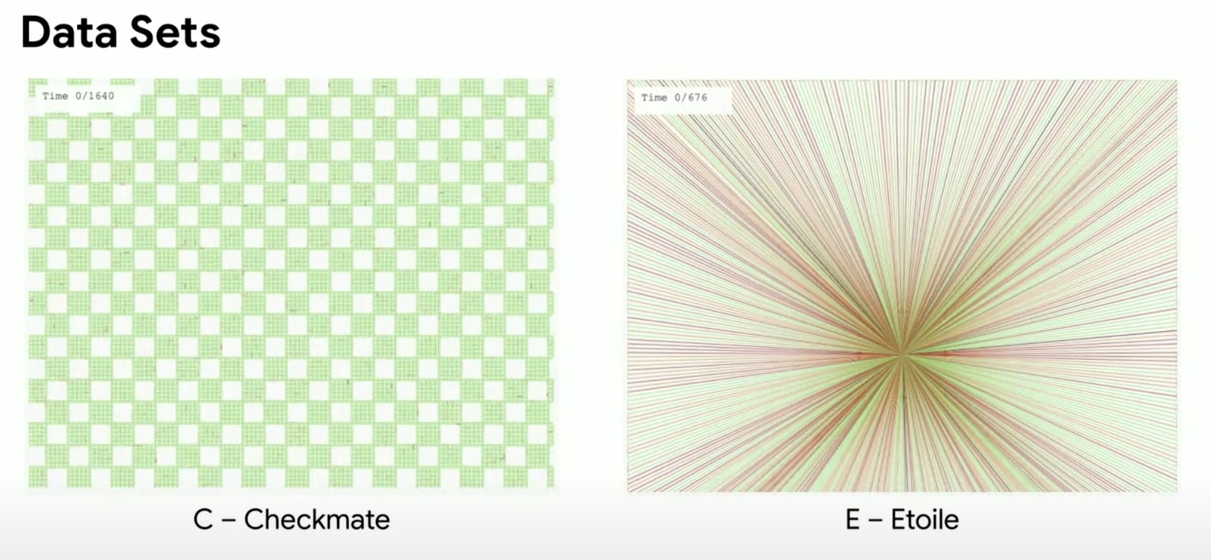
\includegraphics[width=\linewidth]{img/screenshots/hashcode_datasets_c_e.png}
    % 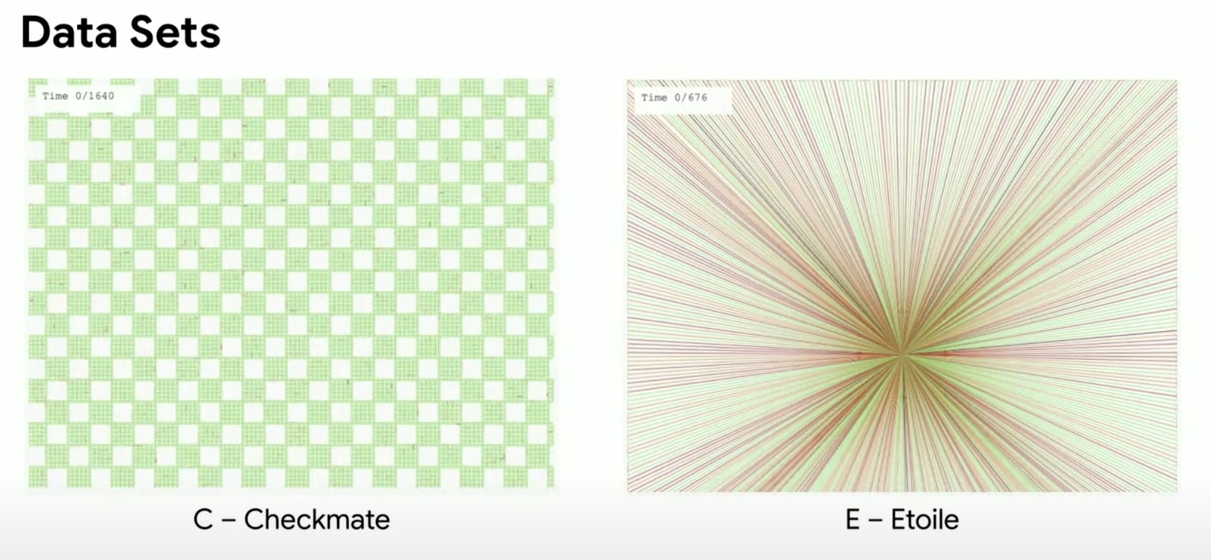
\includegraphics[width=.8\linewidth]{img/screenshots/hashcode_datasets_c_e.png}
    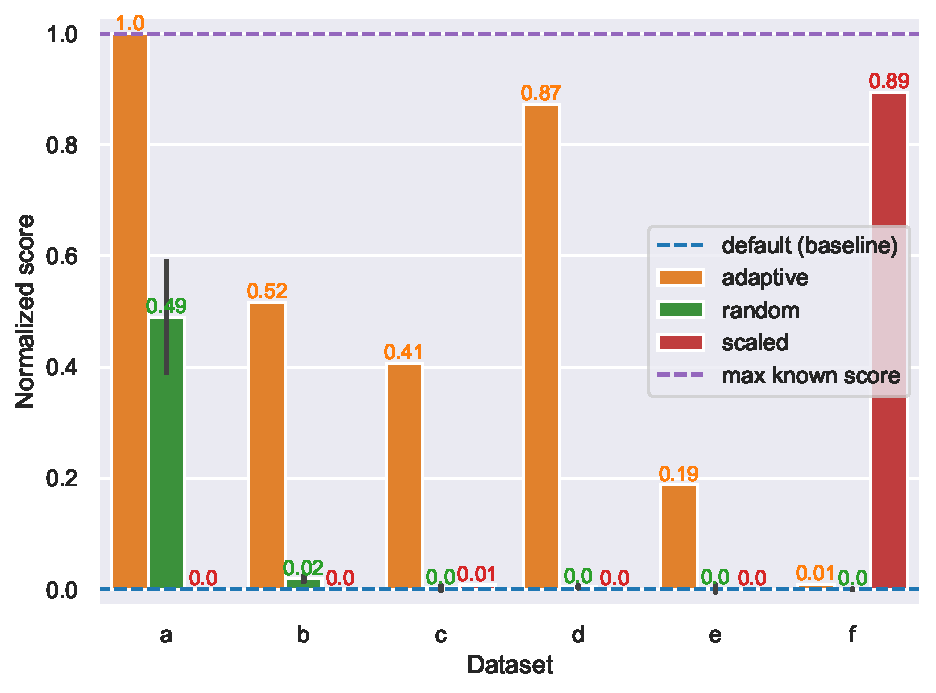
\includegraphics[width=\linewidth]{img/experiments/init_experiment.pdf}
    \caption[Initialization Experiment]{
        Initialization Experiment
    }
    \label{fig:init_experiment}
\end{figure}

\section{Experiment 2: Optimization}

In the second experiment, we compare different optimization methods on datasets B--F. The goal is to find if some method is superior to others or if the ideal method is dataset-dependent. We also want to see how much we can improve from the starting solutions.

\subsection*{Methodology}

We compare the three previously mentioned optimization methods: \textit{genetic algorithm}, \textit{hill climbing} and \textit{simulated annealing}. For each dataset and method, 10 runs with different seeds were performed and averaged to obtain reliable results. ...

\subsection*{Results}
